\section{Обработка табличных данных. Часть 1 (Задание 4 вариант 7)}

\subsection{Условие задания}

Найти среднее арифметическое нечетных элементов, не попадающих в заданный интервал. Вывести номера максимальных нечетных элементов.

Создать приложение для выполнения задания. Использовать элемент формы DataGridView. 

ДИАПАЗОН $[a,b]$ означает, что $mas[i][j] >= a$ \&\& $mas[i][j] <= b$.

Приложение должно выполнять следующие действия:

\begin{enumerate}
    \item{Возможность удалять и добавлять строки таблицы. Проект не должен аварийно завершаться при удалении несуществующей таблицы.}
    \item{Проверять ввод не числовых данных как в таблицу, так и в остальные текстовые поля (если есть в задании).}
    \item{Если есть диапазон значений $[a,b]$, проверять, что $a < b$.}
    \item{Заголовок формы должен отражать суть задания.}
    \item{Все элементы формы должны быть внятно подписаны (кнопки подписаны, у тестового поля должно быть написано, для чего оно нужно и т. д.)}
    \item{В коде должны быть комментарии и отступы (код должен быть легко читаем).}
    \item{В коде программы все элементы формы должны быть переименованы (btnName ---  для кнопок, lblName --- для ссылок, txtName --- для текстового поля и т. д.) Наименования должны быть понятными.}
    \item{Приложение должно корректно работать (выводить ответ или ошибку с соответствующим сообщением). После вывода ошибок при вводе корректных данных поля ошибок должны очищаться.  }
\end{enumerate}

\subsection{Вид формы в конструкторе}

Форма имеет вид как показано на рис.\ref{fig:FormInConstruct4}:

\begin{figure}[!h]
    \centering
    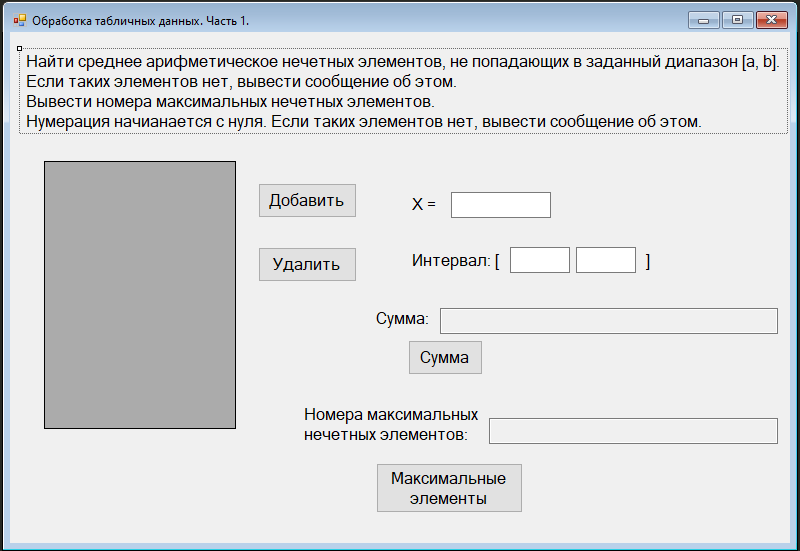
\includegraphics[width = 0.5\textwidth]{images/Task4/FormInConstructor.png}
    \caption{Вид формы в конструкторе}
    \label{fig:FormInConstruct4}
\end{figure}

\newpage
\subsection{Таблица с описанием переименовнных элементов формы}

Все элементы формы были переименованы и их атрибыты изменены. Проведенные изменения представлены в таблице \ref{tab:label4}

\begin{longtable}[!h]{|l|l|l|}
    \caption{Значения атрибутов элементов в приложении <<Обработка табличных данных. Часть 1>>}
    \label{tab:label4}
    \endfirsthead
    \endhead
    \hline
    \makecell{$\textbf{Описание элементов}$\\ $\textbf{формы}$}& \makecell{$\textbf{Список измененных}$\\ $\textbf{атрибутов}$}& \makecell{$\textbf{Новое значение}$\\ $\textbf{атрибута}$}\\ 
    \hline
    \makecell{Форма}& \makecell{Text}& \makecell{Обработка табличных\\ данных 1}\\ 
    \hline
    \makecell{Первая надпись (label)}& \makecell{Name}& \makecell{lblTask}\\ 
    \hline
    \makecell{Первая надпись (label)}& \makecell{Text}& \makecell{Найти среднее\\ арифметическое\\ нечетных элементов,\\не попадающих\\ в заданный\\ диапазон [a, b].\\ Если таких элементов\\ нет, вывести сообщение\\ об этом. Вывести\\ номера максимальных\\ нечетных элементов.\\ Нумерация начианается\\ с нуля. Если таких\\ элементов нет,\\ вывести сообщение\\ об этом.}\\ 
    \hline
    \makecell{Вторая надпись (label)}& \makecell{Name}& \makecell{lblX}\\ 
    \hline
    \makecell{Вторая надпись (label)}& \makecell{Text}& \makecell{X =}\\ 
    \hline
    \makecell{Третья надпись (label)}& \makecell{Name}& \makecell{lblInterval1}\\ 
    \hline
    \makecell{Третья надпись (label)}& \makecell{Text}& \makecell{Интервал: [}\\ 
    \hline
    \makecell{Четвёртая надпись (label)}& \makecell{Name}& \makecell{lblInterval2}\\ 
    \hline
    \makecell{Четвёртая надпись (label)}& \makecell{Text}& \makecell{]}\\ 
    \hline
    \makecell{Пятая надпись (label)}& \makecell{Name}& \makecell{lblSum}\\ 
    \hline
    \makecell{Пятая надпись (label)}& \makecell{Text}& \makecell{Сумма:}\\ 
    \hline
    \makecell{Шестая надпись (label)}& \makecell{Name}& \makecell{lblMaxEl}\\ 
    \hline
    \makecell{Шестая надпись (label)}& \makecell{Text}& \makecell{Номера\\ максимальных\\ нечетных элементов\\}\\ 
    \hline

    \makecell{Первое текстовое\\ поле (textBox)}& \makecell{Name}& \makecell{XTxtBox}\\ 
    \hline
    \makecell{Второе текстовое\\ поле (textBox)}& \makecell{Name}& \makecell{ATxtBox}\\ 
    \hline
    \makecell{Третье текстовое\\ поле (textBox)}& \makecell{Name}& \makecell{BTxtBox}\\ 
    \hline
    \makecell{Четвёртое текстовое\\ поле (textBox)}& \makecell{Name}& \makecell{SumTxtBox}\\ 
    \hline
    \makecell{Четвёртое текстовое\\ поле (textBox)}& \makecell{ReadOnly}& \makecell{True}\\ 
    \hline
    \makecell{Пятое текстовое\\ поле (textBox)}& \makecell{Name}& \makecell{MaxTxtBox}\\ 
    \hline
    \makecell{Пятое текстовое\\ поле (textBox)}& \makecell{ReadOnly}& \makecell{True}\\ 
    \hline

    \makecell{Первая кнопка (button)}& \makecell{Name}& \makecell{AddBtn}\\ 
    \hline
    \makecell{Первая кнопка (button)}& \makecell{Text}& \makecell{Добавить}\\ 
    \hline
    \makecell{Вторая кнопка (button)}& \makecell{Name}& \makecell{DelBtn}\\ 
    \hline
    \makecell{Вторая кнопка (button)}& \makecell{Text}& \makecell{Удалить}\\ 
    \hline
    \makecell{Третья кнопка (button)}& \makecell{Name}& \makecell{SumBtn}\\ 
    \hline
    \makecell{Третья кнопка (button)}& \makecell{Text}& \makecell{Сумма:}\\ 
    \hline
    \makecell{Четвёртая кнопка (button)}& \makecell{Name}& \makecell{MaxBtn}\\ 
    \hline
    \makecell{Четвёртая кнопка (button)}& \makecell{Text}& \makecell{Максимальные\\ элементы}\\ 
    \hline

    \makecell{Таблица (dataGridView)}& \makecell{Name}& \makecell{ArDtGr}\\ 
    \hline

    \makecell{Обработчик ошибок 1\\ (errorProvider)}& \makecell{Name}& \makecell{errPrX}\\ 
    \hline
    \makecell{Обработчик ошибок 2\\ (errorProvider)}& \makecell{Name}& \makecell{errPrA}\\ 
    \hline
    \makecell{Обработчик ошибок 3\\ (errorProvider)}& \makecell{Name}& \makecell{errPrB}\\ 
    \hline
\end{longtable}

\subsection{Примеры работы}

При запуске приложения на экране появляется окно как показано на рис.\ref{fig:StartForm4}.

\newpage

\begin{figure}[!h]
    \centering
    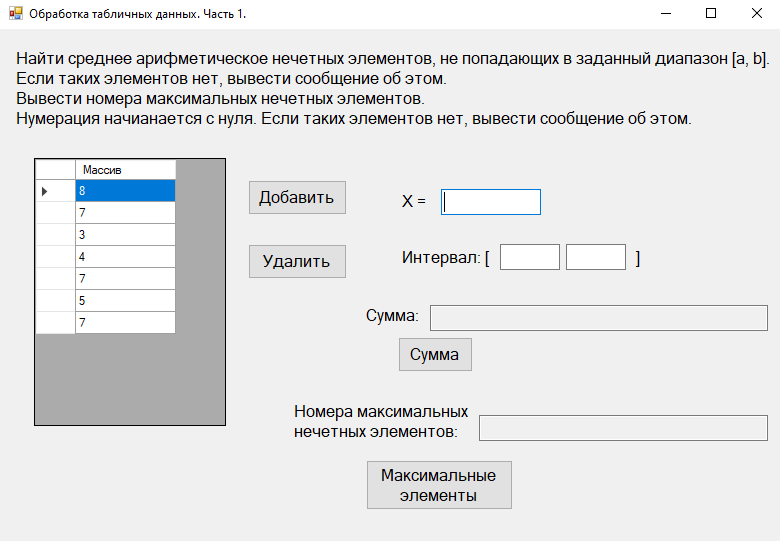
\includegraphics[width = 0.5\textwidth]{images/Task4/Start.png}
    \caption{Запуск приложения}
    \label{fig:StartForm4}
\end{figure}

При запуске с корректными данными, при нажатии на кнопку добавить происходит как показано на рис.\ref{fig:WorkForm4}:

\begin{figure}[!h]
    \centering
    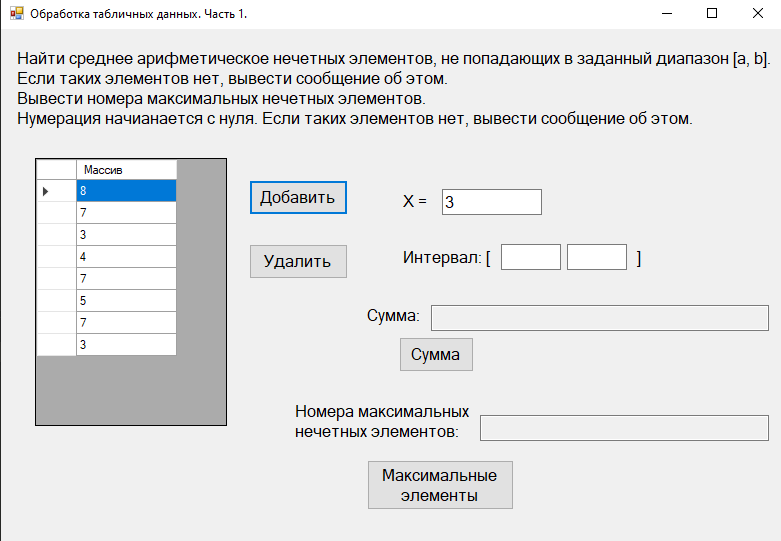
\includegraphics[width = 0.5\textwidth]{images/Task4/WorkAdd.png}
    \caption{Запуск с корректными данными}
    \label{fig:WorkForm4}
\end{figure}

При запуске с некорректными данными, при нажатии на кнопку добавить происходит  как показано на рис.\ref{fig:BadInputNotIntForm4}:

\begin{figure}[!h]
    \centering
    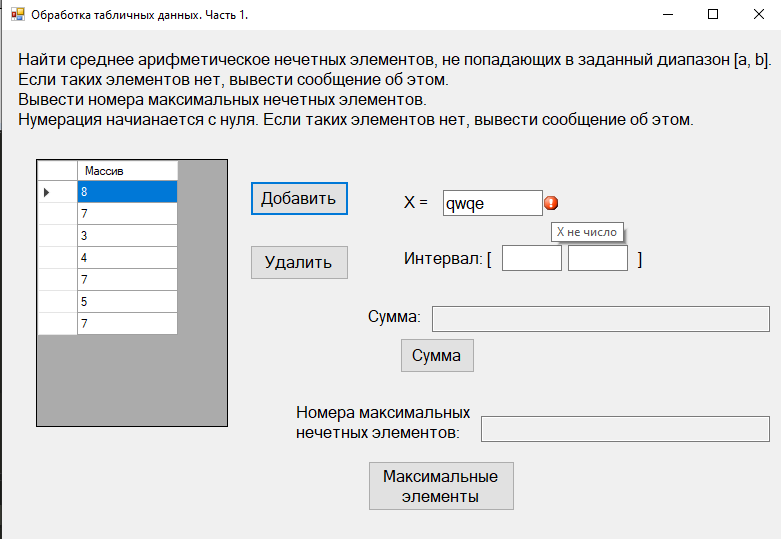
\includegraphics[width = 0.5\textwidth]{images/Task4/BadInputNotIntX.png}
    \caption{Запуск с некорректными данными}
    \label{fig:BadInputNotIntForm4}
\end{figure}

\subsection{Примеры кода}

Функция вставки строки: 

\begin{minted}{c++}
	// вставка строки
	private: System::Void AddBtn_Click(System::Object^ sender, System::EventArgs^ e) {
		ClearAll();
		long long InputX;
		// переводим сторку из TextBox в число
		bool parseX = Int64::TryParse(this->XTxtBox->Text, InputX);
		// ввели не число
		if (!parseX) {
			errPrX->SetError(XTxtBox, "X не число");
		}
		else {
			ArDtGr->Rows->Add();
			ArDtGr->Rows[ArDtGr->RowCount - 1]->Cells[0]->Value = InputX;
		}
	}
\end{minted}

Другие фрагменты кода расположены в приложении \ref{app:task4}. Полный код программы приведен в приложении \ref{app:zip}
